%!TEX root = ./main.tex



\tikzset{every picture/.style={line width=0.75pt}} %set default line width to 0.75pt        

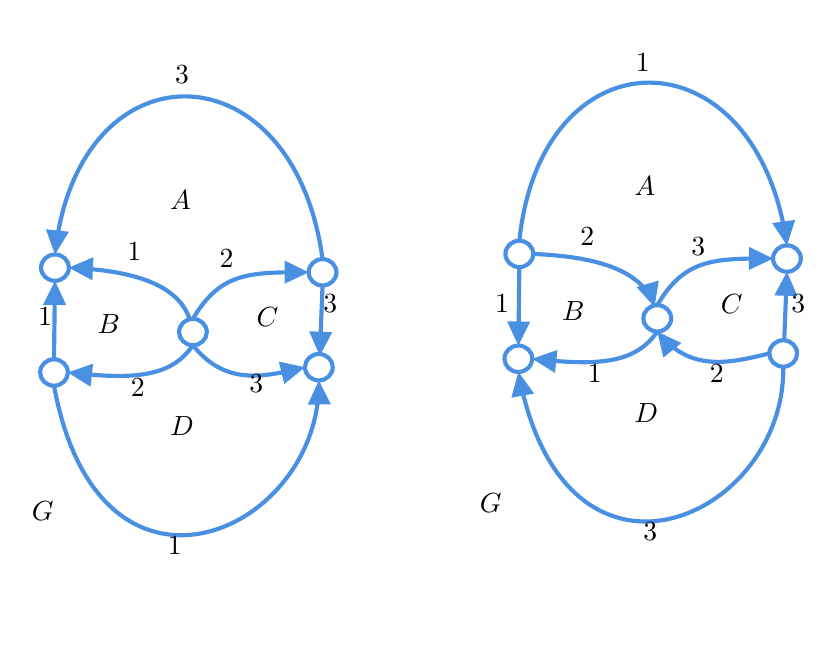
\begin{tikzpicture}[x=0.75pt,y=0.75pt,yscale=-1,xscale=1]
%uncomment if require: \path (0,877); %set diagram left start at 0, and has height of 877

%Straight Lines [id:da9943610350622754] 
\draw [color={rgb, 255:red, 74; green, 144; blue, 226 }  ,draw opacity=1 ][line width=1.5]    (143.18,155.15) -- (143.59,121.34) ;
\draw [shift={(143.64,117.34)}, rotate = 90.69] [fill={rgb, 255:red, 74; green, 144; blue, 226 }  ,fill opacity=1 ][line width=0.08]  [draw opacity=0] (11.61,-5.58) -- (0,0) -- (11.61,5.58) -- cycle    ;
%Straight Lines [id:da28864384570380464] 
\draw [color={rgb, 255:red, 74; green, 144; blue, 226 }  ,draw opacity=1 ][line width=1.5]    (272.57,119.58) -- (271.39,149.46) ;
\draw [shift={(271.23,153.46)}, rotate = 272.26] [fill={rgb, 255:red, 74; green, 144; blue, 226 }  ,fill opacity=1 ][line width=0.08]  [draw opacity=0] (11.61,-5.58) -- (0,0) -- (11.61,5.58) -- cycle    ;
%Shape: Ellipse [id:dp029827328935257524] 
\draw  [color={rgb, 255:red, 74; green, 144; blue, 226 }  ,draw opacity=1 ][fill={rgb, 255:red, 255; green, 255; blue, 255 }  ,fill opacity=1 ][line width=1.5]  (136.95,110.99) .. controls (136.95,107.48) and (139.95,104.64) .. (143.64,104.64) .. controls (147.34,104.64) and (150.33,107.48) .. (150.33,110.99) .. controls (150.33,114.5) and (147.34,117.34) .. (143.64,117.34) .. controls (139.95,117.34) and (136.95,114.5) .. (136.95,110.99) -- cycle ;
%Shape: Ellipse [id:dp4202696786928657] 
\draw  [color={rgb, 255:red, 74; green, 144; blue, 226 }  ,draw opacity=1 ][fill={rgb, 255:red, 255; green, 255; blue, 255 }  ,fill opacity=1 ][line width=1.5]  (136.49,161.51) .. controls (136.49,158) and (139.49,155.15) .. (143.18,155.15) .. controls (146.88,155.15) and (149.88,158) .. (149.88,161.51) .. controls (149.88,165.01) and (146.88,167.86) .. (143.18,167.86) .. controls (139.49,167.86) and (136.49,165.01) .. (136.49,161.51) -- cycle ;
%Shape: Ellipse [id:dp7878916678981432] 
\draw  [color={rgb, 255:red, 74; green, 144; blue, 226 }  ,draw opacity=1 ][fill={rgb, 255:red, 255; green, 255; blue, 255 }  ,fill opacity=1 ][line width=1.5]  (203.42,142.03) .. controls (203.42,138.52) and (206.41,135.67) .. (210.11,135.67) .. controls (213.8,135.67) and (216.8,138.52) .. (216.8,142.03) .. controls (216.8,145.53) and (213.8,148.38) .. (210.11,148.38) .. controls (206.41,148.38) and (203.42,145.53) .. (203.42,142.03) -- cycle ;
%Shape: Ellipse [id:dp9437208822572988] 
\draw  [color={rgb, 255:red, 74; green, 144; blue, 226 }  ,draw opacity=1 ][fill={rgb, 255:red, 255; green, 255; blue, 255 }  ,fill opacity=1 ][line width=1.5]  (265.88,113.23) .. controls (265.88,109.72) and (268.87,106.88) .. (272.57,106.88) .. controls (276.27,106.88) and (279.26,109.72) .. (279.26,113.23) .. controls (279.26,116.74) and (276.27,119.58) .. (272.57,119.58) .. controls (268.87,119.58) and (265.88,116.74) .. (265.88,113.23) -- cycle ;
%Shape: Ellipse [id:dp06226933559817249] 
\draw  [color={rgb, 255:red, 74; green, 144; blue, 226 }  ,draw opacity=1 ][fill={rgb, 255:red, 255; green, 255; blue, 255 }  ,fill opacity=1 ][line width=1.5]  (264.09,158.96) .. controls (264.09,155.46) and (267.09,152.61) .. (270.78,152.61) .. controls (274.48,152.61) and (277.48,155.46) .. (277.48,158.96) .. controls (277.48,162.47) and (274.48,165.32) .. (270.78,165.32) .. controls (267.09,165.32) and (264.09,162.47) .. (264.09,158.96) -- cycle ;
%Curve Lines [id:da2979171995828367] 
\draw [color={rgb, 255:red, 74; green, 144; blue, 226 }  ,draw opacity=1 ][line width=1.5]    (144.19,100.11) .. controls (157.44,2.47) and (258.65,4.55) .. (272.57,106.88) ;
\draw [shift={(143.64,104.64)}, rotate = 275.97] [fill={rgb, 255:red, 74; green, 144; blue, 226 }  ,fill opacity=1 ][line width=0.08]  [draw opacity=0] (11.61,-5.58) -- (0,0) -- (11.61,5.58) -- cycle    ;
%Curve Lines [id:da8764254520788726] 
\draw [color={rgb, 255:red, 74; green, 144; blue, 226 }  ,draw opacity=1 ][line width=1.5]    (154.59,111.21) .. controls (175.51,112.49) and (202.93,116.86) .. (208.77,136.52) ;
\draw [shift={(150.33,110.99)}, rotate = 2.62] [fill={rgb, 255:red, 74; green, 144; blue, 226 }  ,fill opacity=1 ][line width=0.08]  [draw opacity=0] (11.61,-5.58) -- (0,0) -- (11.61,5.58) -- cycle    ;
%Curve Lines [id:da9659495047647262] 
\draw [color={rgb, 255:red, 74; green, 144; blue, 226 }  ,draw opacity=1 ][line width=1.5]    (143.18,167.86) .. controls (164.72,285.2) and (268.93,239.85) .. (270.77,168.59) ;
\draw [shift={(270.78,165.32)}, rotate = 88.95] [fill={rgb, 255:red, 74; green, 144; blue, 226 }  ,fill opacity=1 ][line width=0.08]  [draw opacity=0] (11.61,-5.58) -- (0,0) -- (11.61,5.58) -- cycle    ;
%Curve Lines [id:da5397459745235432] 
\draw [color={rgb, 255:red, 74; green, 144; blue, 226 }  ,draw opacity=1 ][line width=1.5]    (210.11,148.38) .. controls (199.97,163.28) and (183.12,164.92) .. (153.63,161.91) ;
\draw [shift={(149.88,161.51)}, rotate = 6.33] [fill={rgb, 255:red, 74; green, 144; blue, 226 }  ,fill opacity=1 ][line width=0.08]  [draw opacity=0] (11.61,-5.58) -- (0,0) -- (11.61,5.58) -- cycle    ;
%Curve Lines [id:da4211882280413548] 
\draw [color={rgb, 255:red, 74; green, 144; blue, 226 }  ,draw opacity=1 ][line width=1.5]    (210.11,135.67) .. controls (222.75,114.11) and (236.34,113.14) .. (262.15,113.22) ;
\draw [shift={(265.88,113.23)}, rotate = 180.29] [fill={rgb, 255:red, 74; green, 144; blue, 226 }  ,fill opacity=1 ][line width=0.08]  [draw opacity=0] (11.61,-5.58) -- (0,0) -- (11.61,5.58) -- cycle    ;
%Curve Lines [id:da956839943660936] 
\draw [color={rgb, 255:red, 74; green, 144; blue, 226 }  ,draw opacity=1 ][line width=1.5]    (260.12,159.91) .. controls (241.26,164.32) and (224.71,166.59) .. (210.11,148.38) ;
\draw [shift={(264.09,158.96)}, rotate = 166.47] [fill={rgb, 255:red, 74; green, 144; blue, 226 }  ,fill opacity=1 ][line width=0.08]  [draw opacity=0] (11.61,-5.58) -- (0,0) -- (11.61,5.58) -- cycle    ;
%Straight Lines [id:da7109511854568149] 
\draw [color={rgb, 255:red, 74; green, 144; blue, 226 }  ,draw opacity=1 ][line width=1.5]    (366.97,144.53) -- (367.38,110.72) ;
\draw [shift={(366.92,148.53)}, rotate = 270.69] [fill={rgb, 255:red, 74; green, 144; blue, 226 }  ,fill opacity=1 ][line width=0.08]  [draw opacity=0] (11.61,-5.58) -- (0,0) -- (11.61,5.58) -- cycle    ;
%Straight Lines [id:da49493506455500713] 
\draw [color={rgb, 255:red, 74; green, 144; blue, 226 }  ,draw opacity=1 ][line width=1.5]    (496.15,116.96) -- (494.97,146.84) ;
\draw [shift={(496.31,112.96)}, rotate = 92.26] [fill={rgb, 255:red, 74; green, 144; blue, 226 }  ,fill opacity=1 ][line width=0.08]  [draw opacity=0] (11.61,-5.58) -- (0,0) -- (11.61,5.58) -- cycle    ;
%Shape: Ellipse [id:dp9403539709464994] 
\draw  [color={rgb, 255:red, 74; green, 144; blue, 226 }  ,draw opacity=1 ][fill={rgb, 255:red, 255; green, 255; blue, 255 }  ,fill opacity=1 ][line width=1.5]  (360.69,104.37) .. controls (360.69,100.86) and (363.68,98.02) .. (367.38,98.02) .. controls (371.08,98.02) and (374.07,100.86) .. (374.07,104.37) .. controls (374.07,107.88) and (371.08,110.72) .. (367.38,110.72) .. controls (363.68,110.72) and (360.69,107.88) .. (360.69,104.37) -- cycle ;
%Shape: Ellipse [id:dp9543762925369562] 
\draw  [color={rgb, 255:red, 74; green, 144; blue, 226 }  ,draw opacity=1 ][fill={rgb, 255:red, 255; green, 255; blue, 255 }  ,fill opacity=1 ][line width=1.5]  (360.23,154.89) .. controls (360.23,151.38) and (363.23,148.53) .. (366.92,148.53) .. controls (370.62,148.53) and (373.62,151.38) .. (373.62,154.89) .. controls (373.62,158.39) and (370.62,161.24) .. (366.92,161.24) .. controls (363.23,161.24) and (360.23,158.39) .. (360.23,154.89) -- cycle ;
%Shape: Ellipse [id:dp6094250043745837] 
\draw  [color={rgb, 255:red, 74; green, 144; blue, 226 }  ,draw opacity=1 ][fill={rgb, 255:red, 255; green, 255; blue, 255 }  ,fill opacity=1 ][line width=1.5]  (427.15,135.41) .. controls (427.15,131.9) and (430.15,129.06) .. (433.85,129.06) .. controls (437.54,129.06) and (440.54,131.9) .. (440.54,135.41) .. controls (440.54,138.92) and (437.54,141.76) .. (433.85,141.76) .. controls (430.15,141.76) and (427.15,138.92) .. (427.15,135.41) -- cycle ;
%Shape: Ellipse [id:dp7048265837255207] 
\draw  [color={rgb, 255:red, 74; green, 144; blue, 226 }  ,draw opacity=1 ][fill={rgb, 255:red, 255; green, 255; blue, 255 }  ,fill opacity=1 ][line width=1.5]  (489.62,106.61) .. controls (489.62,103.1) and (492.61,100.26) .. (496.31,100.26) .. controls (500,100.26) and (503,103.1) .. (503,106.61) .. controls (503,110.12) and (500,112.96) .. (496.31,112.96) .. controls (492.61,112.96) and (489.62,110.12) .. (489.62,106.61) -- cycle ;
%Shape: Ellipse [id:dp8750927184704229] 
\draw  [color={rgb, 255:red, 74; green, 144; blue, 226 }  ,draw opacity=1 ][fill={rgb, 255:red, 255; green, 255; blue, 255 }  ,fill opacity=1 ][line width=1.5]  (487.83,152.35) .. controls (487.83,148.84) and (490.83,145.99) .. (494.52,145.99) .. controls (498.22,145.99) and (501.22,148.84) .. (501.22,152.35) .. controls (501.22,155.85) and (498.22,158.7) .. (494.52,158.7) .. controls (490.83,158.7) and (487.83,155.85) .. (487.83,152.35) -- cycle ;
%Curve Lines [id:da5236484284848602] 
\draw [color={rgb, 255:red, 74; green, 144; blue, 226 }  ,draw opacity=1 ][line width=1.5]    (367.38,98.02) .. controls (377.97,-3.17) and (480.11,-3.63) .. (495.86,97.17) ;
\draw [shift={(496.31,100.26)}, rotate = 262.26] [fill={rgb, 255:red, 74; green, 144; blue, 226 }  ,fill opacity=1 ][line width=0.08]  [draw opacity=0] (11.61,-5.58) -- (0,0) -- (11.61,5.58) -- cycle    ;
%Curve Lines [id:da9662673859391505] 
\draw [color={rgb, 255:red, 74; green, 144; blue, 226 }  ,draw opacity=1 ][line width=1.5]    (374.07,104.37) .. controls (394.05,105.28) and (422.58,108.46) .. (431.12,126.3) ;
\draw [shift={(432.51,129.9)}, rotate = 253.46] [fill={rgb, 255:red, 74; green, 144; blue, 226 }  ,fill opacity=1 ][line width=0.08]  [draw opacity=0] (11.61,-5.58) -- (0,0) -- (11.61,5.58) -- cycle    ;
%Curve Lines [id:da48834267482785687] 
\draw [color={rgb, 255:red, 74; green, 144; blue, 226 }  ,draw opacity=1 ][line width=1.5]    (367.96,166.49) .. controls (391.97,278.91) and (495.84,230.72) .. (494.52,158.7) ;
\draw [shift={(366.92,161.24)}, rotate = 79.6] [fill={rgb, 255:red, 74; green, 144; blue, 226 }  ,fill opacity=1 ][line width=0.08]  [draw opacity=0] (11.61,-5.58) -- (0,0) -- (11.61,5.58) -- cycle    ;
%Curve Lines [id:da8150566103908512] 
\draw [color={rgb, 255:red, 74; green, 144; blue, 226 }  ,draw opacity=1 ][line width=1.5]    (433.85,141.76) .. controls (423.71,156.66) and (406.86,158.3) .. (377.37,155.29) ;
\draw [shift={(373.62,154.89)}, rotate = 6.33] [fill={rgb, 255:red, 74; green, 144; blue, 226 }  ,fill opacity=1 ][line width=0.08]  [draw opacity=0] (11.61,-5.58) -- (0,0) -- (11.61,5.58) -- cycle    ;
%Curve Lines [id:da4757930219164036] 
\draw [color={rgb, 255:red, 74; green, 144; blue, 226 }  ,draw opacity=1 ][line width=1.5]    (433.85,129.06) .. controls (446.49,107.49) and (460.08,106.52) .. (485.88,106.6) ;
\draw [shift={(489.62,106.61)}, rotate = 180.29] [fill={rgb, 255:red, 74; green, 144; blue, 226 }  ,fill opacity=1 ][line width=0.08]  [draw opacity=0] (11.61,-5.58) -- (0,0) -- (11.61,5.58) -- cycle    ;
%Curve Lines [id:da9886701870479793] 
\draw [color={rgb, 255:red, 74; green, 144; blue, 226 }  ,draw opacity=1 ][line width=1.5]    (487.83,152.35) .. controls (468.44,157.01) and (451.43,160.8) .. (436.44,144.76) ;
\draw [shift={(433.85,141.76)}, rotate = 51.28] [fill={rgb, 255:red, 74; green, 144; blue, 226 }  ,fill opacity=1 ][line width=0.08]  [draw opacity=0] (11.61,-5.58) -- (0,0) -- (11.61,5.58) -- cycle    ;

% Text Node
\draw (197.61,72.18) node [anchor=north west][inner sep=0.75pt]    {$A$};
% Text Node
\draw (162.72,132.26) node [anchor=north west][inner sep=0.75pt]    {$B$};
% Text Node
\draw (239.25,128.92) node [anchor=north west][inner sep=0.75pt]    {$C$};
% Text Node
\draw (197.61,181.41) node [anchor=north west][inner sep=0.75pt]    {$D$};
% Text Node
\draw (196.52,239.02) node [anchor=north west][inner sep=0.75pt]    {$1$};
% Text Node
\draw (221.51,100.97) node [anchor=north west][inner sep=0.75pt]    {$2$};
% Text Node
\draw (200.09,12.4) node [anchor=north west][inner sep=0.75pt]    {$3$};
% Text Node
\draw (235.78,161.1) node [anchor=north west][inner sep=0.75pt]    {$3$};
% Text Node
\draw (177,97.4) node [anchor=north west][inner sep=0.75pt]    {$1$};
% Text Node
\draw (134.06,128.92) node [anchor=north west][inner sep=0.75pt]    {$1$};
% Text Node
\draw (178.68,162.8) node [anchor=north west][inner sep=0.75pt]    {$2$};
% Text Node
\draw (271.48,122.5) node [anchor=north west][inner sep=0.75pt]    {$3$};
% Text Node
\draw (421.34,65.56) node [anchor=north west][inner sep=0.75pt]    {$A$};
% Text Node
\draw (386.46,125.64) node [anchor=north west][inner sep=0.75pt]    {$B$};
% Text Node
\draw (462.98,122.3) node [anchor=north west][inner sep=0.75pt]    {$C$};
% Text Node
\draw (421.34,174.79) node [anchor=north west][inner sep=0.75pt]    {$D$};
% Text Node
\draw (354.23,122.3) node [anchor=north west][inner sep=0.75pt]    {$1$};
% Text Node
\draw (398.85,156.18) node [anchor=north west][inner sep=0.75pt]    {$1$};
% Text Node
\draw (395.28,90.12) node [anchor=north west][inner sep=0.75pt]    {$2$};
% Text Node
\draw (497,122.3) node [anchor=north west][inner sep=0.75pt]    {$3$};
% Text Node
\draw (422.05,6.28) node [anchor=north west][inner sep=0.75pt]    {$1$};
% Text Node
\draw (457.74,156.18) node [anchor=north west][inner sep=0.75pt]    {$2$};
% Text Node
\draw (425.62,232.4) node [anchor=north west][inner sep=0.75pt]    {$3$};
% Text Node
\draw (448.82,95.2) node [anchor=north west][inner sep=0.75pt]    {$3$};
% Text Node
\draw (131,222.4) node [anchor=north west][inner sep=0.75pt]    {$G$};
% Text Node
\draw (346.85,218.4) node [anchor=north west][inner sep=0.75pt]    {$G$};


\end{tikzpicture}